%===============================================================================
\begin{frame}
\frametitle{Архитектура нейронной сети}
\begin{columns}[T]
    \column{1\textwidth}
    
    \begin{block}{\centering Архитектура НС}
        \vspace{1mm}
        \centering 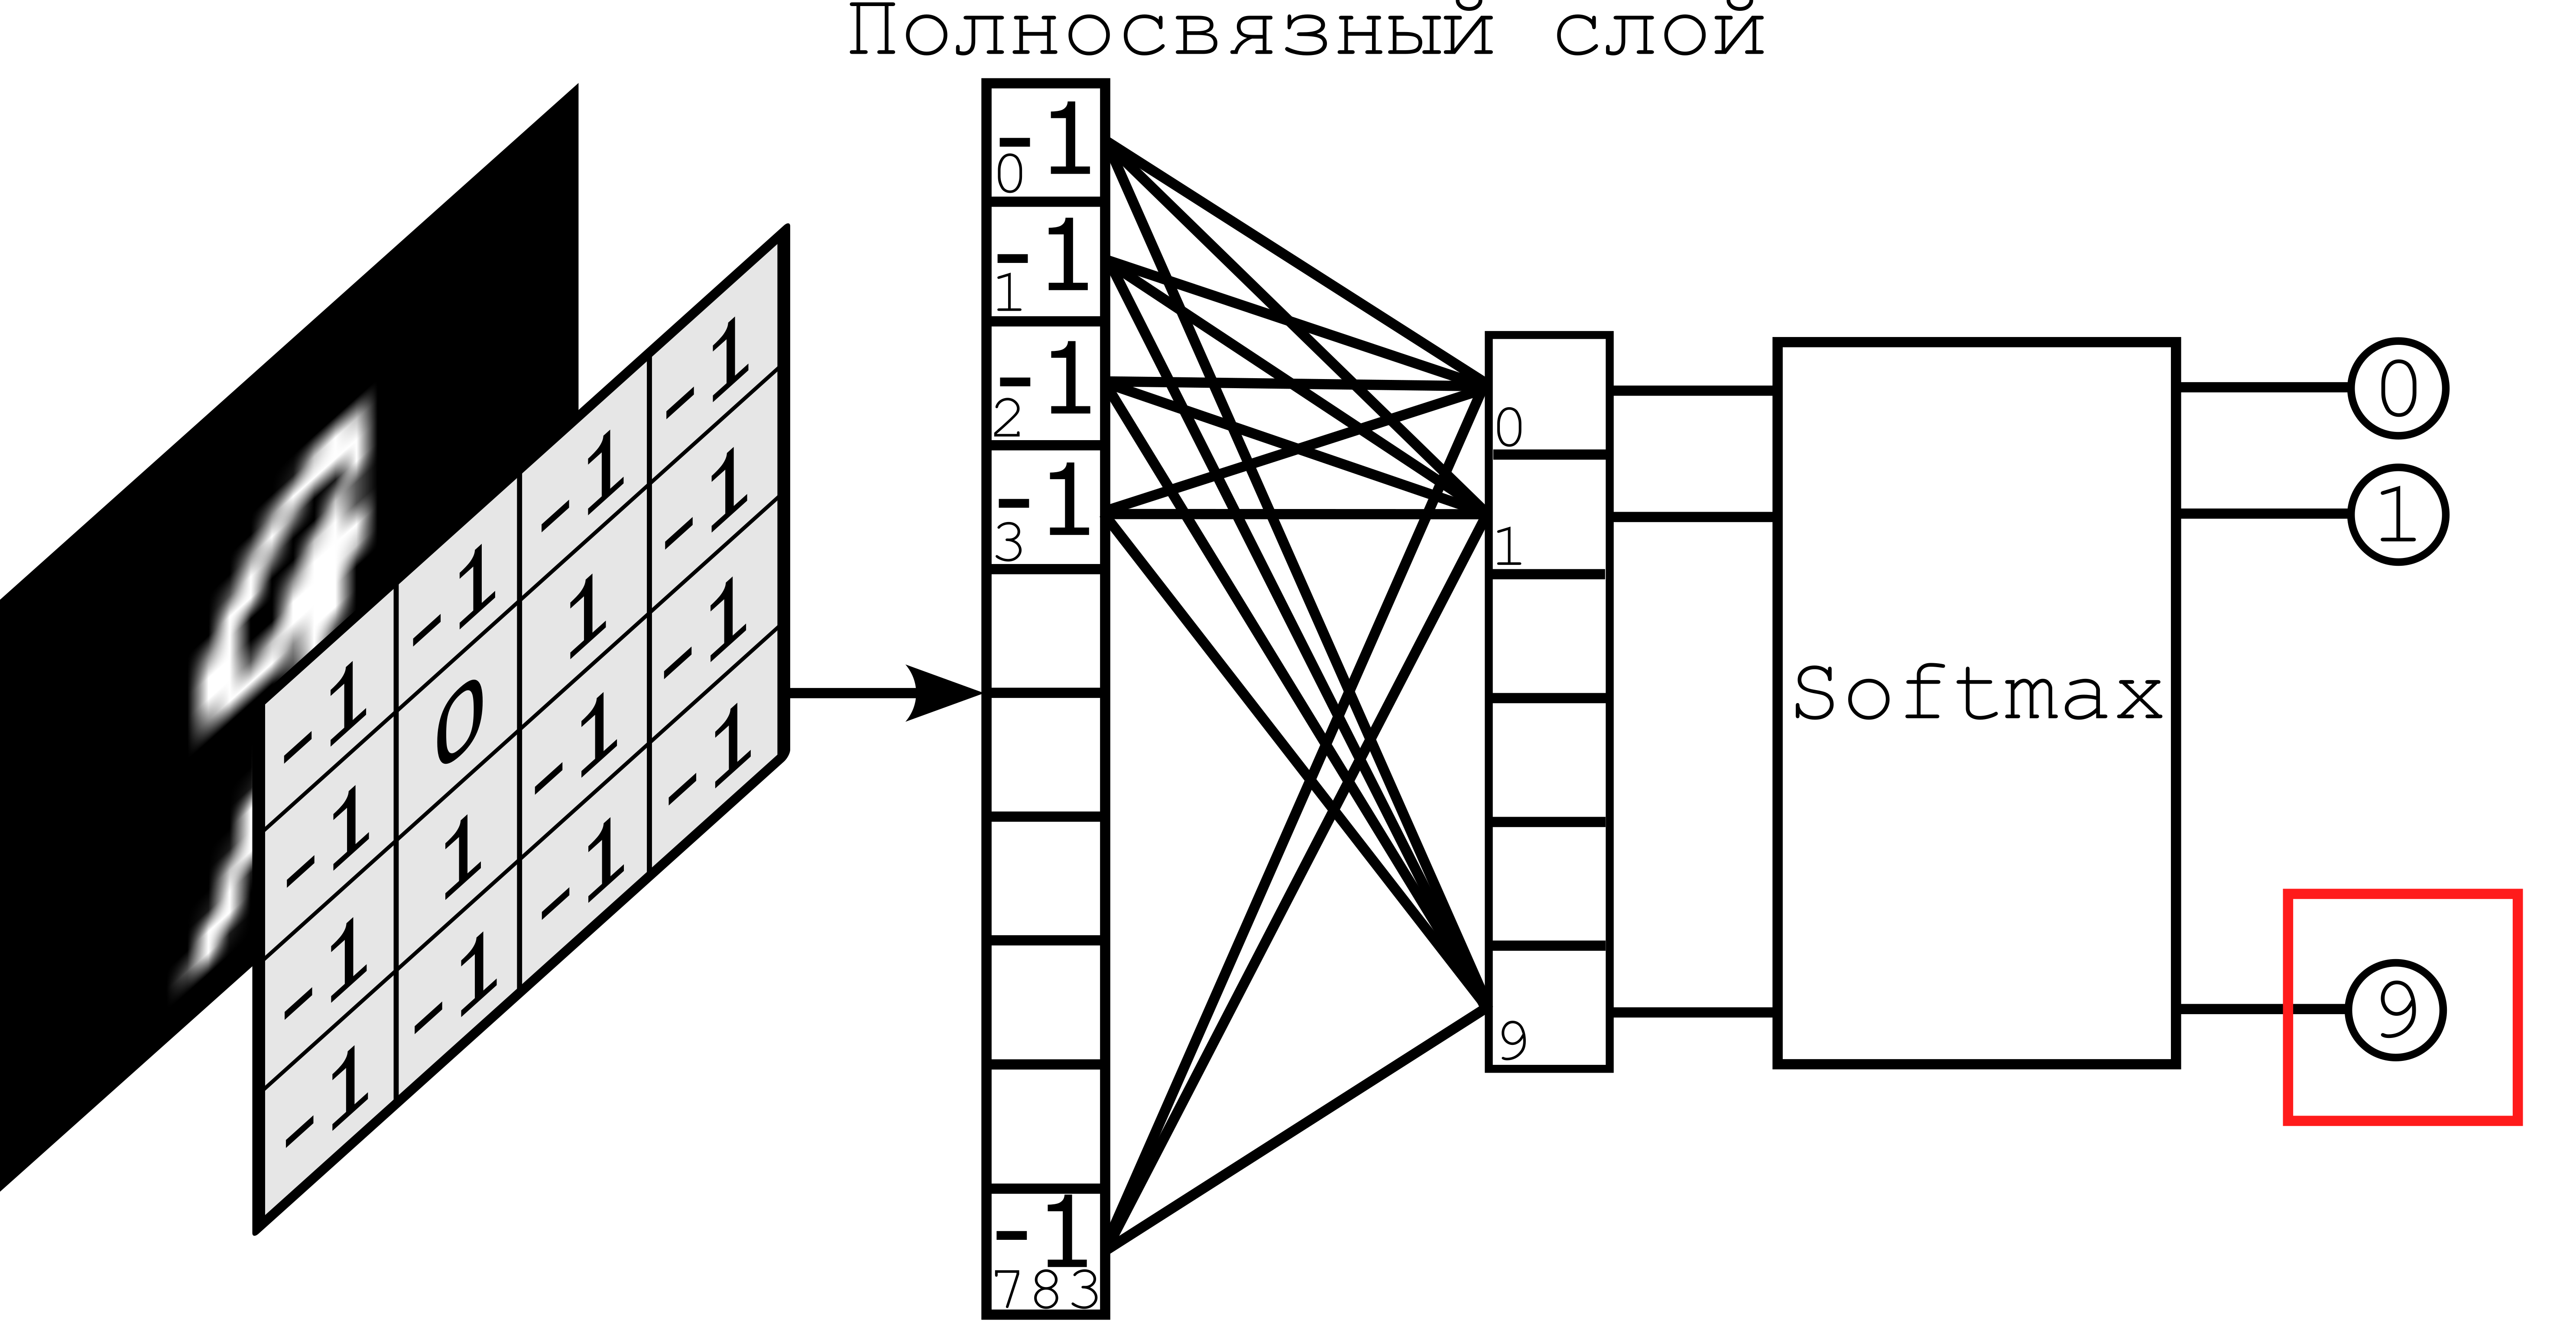
\includegraphics[width = 0.7\textwidth]{pics/nn.png}
        % \includesvg[height = 0.4\textheight]{basic_AE.svg}        
    \end{block}        

    \column{1\textwidth}
    \vspace{-2mm}
        
\end{columns}
\end{frame}
%===============================================================================
\begin{frame}[t]
    \frametitle{Параметры НС}
    \begin{itemize}
        \item Входные данные приводятся к диапазону [-1, 1] и устанавливается их
        среднеквадратическое отклонение(СКО) равным 0,5
        \item Оптимизация производилось с использованием метода стохастического градиентного спуска (SGD)
        (скорость обучения $\eta =3 \cdot 10^{-3}$, число эпох -- 10000, моментум $\gamma = 0,9$)
        \item Для оценки качества декодирования изображений использовались 
        метрика $MSE$
    \end{itemize}
    
    \end{frame}
    